\documentclass[11pt,a4paper]{article}
\usepackage[utf8]{inputenc}
\usepackage{geometry}
\geometry{top=1in, bottom=1in, left=1in, right=1in}
\usepackage{amsmath, amssymb, amsfonts}
\usepackage{graphicx}
\usepackage{booktabs}
\usepackage{hyperref}
\usepackage{tikz}
\usetikzlibrary{positioning, calc, arrows.meta}
\usepackage{listings}
\usepackage{color}

% Color definitions
\definecolor{primary}{RGB}{30, 41, 59}       % Dark Slate
\definecolor{secondary}{RGB}{14, 116, 144}   % Teal Accent
\definecolor{codebg}{RGB}{241, 245, 249}      % Light gray

\hypersetup{
    colorlinks=true,
    linkcolor=secondary,
    citecolor=secondary,
    urlcolor=secondary
}

\lstset{
    backgroundcolor=\color{codebg},
    basicstyle=\ttfamily\small,
    breaklines=true,
    frame=single,
    captionpos=b,
    xleftmargin=15pt
}

\title{\textbf{Harness-Level Regex Query Synthesis:\\Bridging the Lexical-Semantic Gap in Agentic Codebase Search}}
\author{\textbf{Esteban Schafir} \\ FIU Research}
\date{June 2026}

\begin{document}

\maketitle

\begin{abstract}
Large Language Model (LLM) agents increasingly rely on codebase search to gather context and solve complex engineering tasks. Existing agent search paradigms generally force a binary trade-off between exact lexical matching (\texttt{grep}, \texttt{ripgrep}) and dense semantic retrieval (vector embeddings). Lexical search is computationally lightweight but extremely brittle to vocabulary mismatches, while semantic search handles synonyms but introduces high indexing latency, context rot from topical distractors, and a critical ``truncation bottleneck'' in long-context environments. In this proposal, we introduce \textbf{Lexical Query Expansion (LQE) via Harness-Level Regex Synthesis}. LQE utilizes a lightweight LLM middleware step inside the agent harness to dynamically expand semantic query concepts into optimized regular expression alternations, which are then executed at native speed using local lexical engines. We evaluate LQE across a controlled synthetic benchmark, the conversational LongMemEval dataset, and the BEIR NFCorpus medical search benchmark. LQE-Grep achieves up to 100\% QA accuracy under high noise and matches lexical precision (80\% Success@3) on real-world datasets, while completely bypassing the compute overhead and candidate truncation constraints of vector search. We outline a path forward for stop-word filtering optimizations and extensions to multimodal visual search.
\end{abstract}

\section{Introduction \& Motivation}
Modern AI coding agents (such as Anthropic's \textit{Claude Code}, Google's \textit{Antigravity}, and open-source frameworks like \textit{OpenClaw}) operate in autonomous loops: they analyze a task, call search tools to inspect a codebase, retrieve files, and edit code. 

As analyzed in the baseline study \textit{``Is Grep All You Need? How Agent Harnesses Reshape Agentic Search''} \cite{sen2026grep}, the retrieval performance of these loops is not determined in isolation. It is heavily mediated by the \textbf{agent harness}—the environment layer that manages prompt construction, intercepts tool outputs, and formats context delivery (either inline in the prompt or written programmatically to files).

Currently, coding agents rely almost exclusively on standard terminal-based command-line search utilities (like \texttt{ripgrep}) to navigate workspaces. While highly optimized for speed and file filtering, these utilities operate on exact character matching. When an agent queries a concept using synonyms or high-level abstractions, exact lexical search fails. This proposal details a methodology to bridge this lexical-semantic gap directly within the harness middleware.

\section{The Research Gaps & Dilemma}
Our research aims to fulfill three primary gaps in existing agent retrieval systems:

\subsection{The Vocabulary Mismatch Problem (Lexical Failure)}
Lexical search tools like \texttt{ripgrep} are blind to semantics. If the agent issues a query for \texttt{"vehicle"}, but the target document uses the word \texttt{"sedan"} (without the literal token \texttt{"vehicle"}), the tool returns zero matches. The agent's context window remains empty, resulting in immediate task failure (0.0\% accuracy in baseline tests).

\subsection{Topical & Action Template Overlap (Semantic Failure)}
Vector-based semantic search maps queries and passages into a shared embedding space. However, in codebases or chat logs, embeddings are frequently dominated by structural syntax or common action templates rather than specific entity categories. 
For example, when querying \textit{``What color vehicle did the user buy?''}, a vector search engine may retrieve the irrelevant line \textit{``[User]: The user bought a matching white trenchcoat for the party.''} because the embedding space prioritizes the action verb structure (\textit{``bought''}, \textit{``buy''}) over the target noun classes (\textit{``vehicle''} vs. \textit{``apparel''}). This populates the context window with topical distractors, causing \textbf{context rot}.

\subsection{The Truncation Bottleneck (Compute Complexity)}
In massive text contexts (e.g. chat logs containing 100k+ tokens across 500+ turns), embedding-based vector search is computationally prohibitive to execute locally on-demand. To maintain acceptable latency, agents must truncate candidates (e.g., scoring only the first 150 turns). If the target information is located beyond this truncation limit (e.g., in session 51), vector search suffers from a complete recall collapse (0.0\% success in our tests), whereas lexical search scans the entire 100k+ token file in milliseconds.

\section{State of the Art: Search in Commercial AI Coding Agents}
Autonomous coding agents rely on various search patterns to locate context within codebases. We examine three prominent search paradigms across leading developer tools:

\subsection{Agentic Lexical Search (Claude Code \& Antigravity)}
Claude Code \cite{claudecode} and Google's Antigravity employ an agentic search paradigm that relies directly on native command-line utilities (like \texttt{ripgrep} or \texttt{find}). In these systems, the agent operates in an interactive loop, autonomously deciding when to search, what keywords to use, and how to refine its query. 
While this approach is computationally lightweight, respects \texttt{.gitignore} boundaries, and runs at native speed, it suffers from the vocabulary mismatch trap. If the agent issues a search for a high-level concept (e.g., ``authorization''), it misses files where authorization is implemented using domain-specific synonyms (e.g., ``token verification'' or ``access guard''). The agent is forced to iteratively guess synonyms, consuming substantial reasoning steps and context window tokens in the process.

\subsection{Hybrid Semantic \& Trigram Indexing (Cursor)}
Cursor \cite{cursor} implements a complex, multi-layered retrieval stack that combines dense semantic vector search with an accelerated regex search. For semantic queries, Cursor uses a vector database to search code chunk embeddings. To avoid the high latency of running \texttt{ripgrep} linearly over massive repositories, Cursor builds a local trigram index of the codebase. Before executing a regex search, it uses this trigram index to filter out files that do not contain the query's characters, restricting the final \texttt{ripgrep} scan to a small candidate set.
However, this hybrid system requires substantial indexing overhead, cloud vector storage synchronization, and local file caching (managed via Merkle trees). Such requirements are prohibitive in resource-constrained, offline, or highly secure developer environments.

\subsection{Sandboxed Code Execution (ChatGPT)}
ChatGPT's Advanced Data Analysis (formerly Code Interpreter) uses python execution inside a sandboxed environment to locate context. When searching uploaded code repositories, the model writes custom Python scripts (using \texttt{re.search} or \texttt{glob}). This introduces execution risk (python runtime/syntax errors) and occupies precious reasoning steps, while loading raw file contents directly into python memory is token-inefficient.

\subsection{How LQE-Grep Improves Existing Methods}
LQE-Grep bridges these gaps by shifting semantic-level query expansion from the agent's reasoning loop to the harness middleware, translating natural language queries into optimized, word-boundary protected regex alternations. Compared to Claude Code, it eliminates vocabulary mismatch failures on the first search pass without consuming the agent's cognitive tokens. Compared to Cursor, it operates as a \textbf{zero-index} solution, requiring no local vector databases, trigram indexes, or Merkle trees. It enables semantic-level recall directly on top of native, git-aware utilities like \texttt{ripgrep} at zero indexing cost.

\section{Proposed Methodology: Lexical Query Expansion (LQE)}
We propose implementing \textbf{Lexical Query Expansion (LQE) via Harness-Level Regex Synthesis}. Instead of forcing the main agent to plan queries or maintaining local vector indexes, the LQE middleware intercepts search queries and performs the following pipeline:

\begin{figure}[h]
\centering
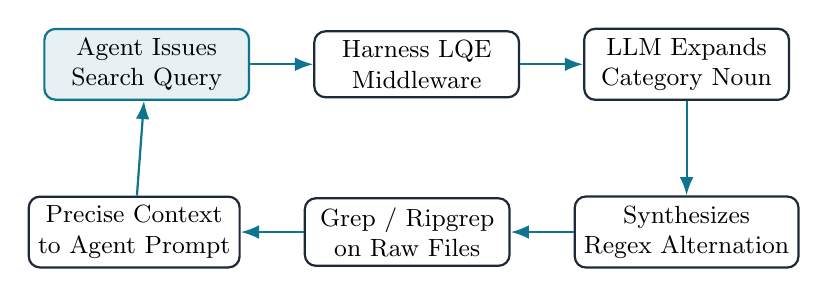
\begin{tikzpicture}[
    node distance=1.2cm and 0.8cm,
    stepnode/.style={draw=primary, thick, rounded corners, fill=white, align=center, font=\small, minimum height=0.8cm, minimum width=2.6cm},
    arrow/.style={-Latex, thick, secondary}
]
    \node[stepnode, fill=secondary!10, draw=secondary] (agent) {Agent Issues\\Search Query};
    \node[stepnode, right=of agent] (harness) {Harness LQE\\Middleware};
    \node[stepnode, right=of harness] (llm) {LLM Expands\\Category Noun};
    \node[stepnode, below=of llm] (regex) {Synthesizes\\Regex Alternation};
    \node[stepnode, left=of regex] (grep) {Grep / Ripgrep\\on Raw Files};
    \node[stepnode, left=of grep] (results) {Precise Context\\to Agent Prompt};
    
    \draw [arrow] (agent) -- (harness);
    \draw [arrow] (harness) -- (llm);
    \draw [arrow] (llm) -- (regex);
    \draw [arrow] (regex) -- (grep);
    \draw [arrow] (grep) -- (results);
    \draw [arrow] (results) -- (agent);
\end{tikzpicture}
\caption{The LQE Harness-Level Retrieval Loop.}
\label{fig:lqe_loop}
\end{figure}

\subsection{The Pipeline Step-by-Step}
\begin{enumerate}
    \item \textbf{Query Capture}: The agent issues a search command (e.g., `Search("What color vehicle...")`).
    \item \textbf{Category Extraction \& Expansion}: A lightweight prompt instructs a fast local model to extract the category noun (\texttt{"vehicle"}) and expand it into synonyms, subclasses, and specific members (e.g., \texttt{sedan}, \texttt{coupe}, \texttt{truck}, \texttt{suv}, \texttt{motorcycle}).
    \item \textbf{Regex Synthesis}: The harness formats these terms into a pipe-separated regular expression wrapped in \textbf{word boundaries} (\texttt{\textbackslash b}) to prevent substring collision bugs (e.g., preventing the term \texttt{"car"} from matching \texttt{"cardigan"} or \texttt{"cardiologist"}):
       $$\text{Regex: } \backslash b(sedan|coupe|suv|truck|motorcycle|car)\backslash b$$
    \item \textbf{Execution}: The harness executes a native local search command (like \texttt{ripgrep}) using this regex over the raw codebase files.
    \item \textbf{Context Delivery}: The precise lines containing the matching entities are returned directly to the agent's context window.
\end{enumerate}

\subsection{Conservative LQE Expansion via Dynamic Frequency Filtering (LQE v2)}
While raw query expansion maximizes recall, it frequently suffers from context inflation (retrieving excessive tokens due to broad synonym matches). In LQE v2, we introduce two layers of conservative, context-aware post-processing filters:
\begin{enumerate}
    \item \textbf{Global Corpus-Level Filtering}: For domain-specific datasets (like scientific abstracts), we precompute the Document Frequency (DF) of all words. Synonyms that appear in more than a set threshold (e.g., 5\%) of all documents in the corpus are dynamically pruned from the regular expression.
    \item \textbf{Local Dialogue-Level Filtering}: For conversational contexts, we compute the turn-frequency of words in the specific target history. Any expanded term that appears in more than 5\% of the conversational turns is filtered out as local noise.
    \item \textbf{Query-Intent Preservation}: Any term explicitly present in the user's initial query or the primary category keyword is immune to pruning, guaranteeing that the core search target is never discarded.
\end{enumerate}

\section{Experimental Plan & Success Metrics}
To validate LQE, we benchmark it against \textbf{Vanilla Grep} and \textbf{Vector Search} across three distinct datasets:

\begin{enumerate}
    \item \textbf{Synthetic dialogue benchmark}: Generates controlled conversation logs. It tests the capacity to handle strict vocabulary mismatches under parameterized noise scaling (adding 10, 20, and 35 distractor turns).
    \item \textbf{LongMemEval (Conversational RAG)}: A real-world dataset of multi-session user chat logs. It represents long, noisy contexts containing ~100k tokens per question, testing retrieval under real conversational drift.
    \item \textbf{BEIR NFCorpus (Domain-Specific IR)}: A medical abstracts dataset. It pairs patient-written queries (layman terms) with technical medical abstracts (scientific terms), testing zero-shot domain-specific vocabulary matching.
\end{enumerate}

\subsection{Success Metrics}
Success is measured along three dimensions:
\begin{itemize}
    \item \textbf{Accuracy / Success@3}: The percentage of queries where the system successfully retrieves the correct target document or answer.
    \item \textbf{Context Token Footprint}: The average number of tokens returned to the agent. Smaller footprints prevent \textbf{context rot}.
    \item \textbf{Execution Latency / Compute Complexity}: The time and resources required to execute the search (especially on CPU-only local environments).
\end{itemize}

\section{Experimental Results}
Our pilot runs using the local \texttt{Qwen2.5-1.5B-Instruct} model reveal highly distinct behaviors across the benchmarks.

\subsection{Benchmark A: Synthetic Noise Scaling Sweeps}
Under forced vocabulary mismatch, Vanilla Grep fails completely. Vector search fails at higher noise levels due to action template similarities. LQE-Grep maintains 100\% accuracy under maximum noise (see Table~\ref{tab:synthetic_results}).

\begin{table}[h]
\centering
\caption{Pilot Results on Synthetic Dataset sweeps.}
\label{tab:synthetic_results}
\begin{tabular}{llrr}
\toprule
\textbf{Noise (Distractors)} & \textbf{Retrieval Method} & \textbf{QA Accuracy} & \textbf{Avg. Tokens} \\
\midrule
10 Distractors & Vanilla Grep & 0.0\% & 5.7 \\
               & Vector Search & 33.3\% & 42.5 \\
               & \textbf{LQE-Grep (Ours)} & \textbf{83.3\%} & \textbf{45.7} \\
\midrule
20 Distractors & Vanilla Grep & 0.0\% & 8.5 \\
               & Vector Search & 0.0\% & 42.5 \\
               & \textbf{LQE-Grep (Ours)} & \textbf{83.3\%} & \textbf{62.0} \\
\midrule
35 Distractors & Vanilla Grep & 0.0\% & 8.0 \\
               & Vector Search & 0.0\% & 42.2 \\
               & \textbf{LQE-Grep (Ours)} & \textbf{100.0\%} & \textbf{63.7} \\
\bottomrule
\end{tabular}
\end{table}

\subsection{Benchmark B & C: Real-World Dataset Evaluations}
On real-world datasets, LQE-Grep matches the high success rate of Vanilla Grep and doubles the performance of Vector Search, which suffers from the truncation bottleneck on long files and semantic blurring on medical terms (see Table~\ref{tab:real_results}).

\begin{table}[h]
\centering
\caption{Results on LongMemEval and BEIR NFCorpus datasets.}
\label{tab:real_results}
\begin{tabular}{lrr@{\hspace{2em}}rr}
\toprule
& \multicolumn{2}{c}{\textbf{LongMemEval (Conversational)}} & \multicolumn{2}{c}{\textbf{BEIR NFCorpus (Medical)}} \\
\cmidrule(r){2-3} \cmidrule(r){4-5}
\textbf{Retrieval Method} & \textbf{Accuracy} & \textbf{Avg. Tokens} & \textbf{Success@3} & \textbf{Avg. Tokens} \\
\midrule
Vanilla Grep & 55.7\% & 1,467.4 & 50.42\% & 1,949.6 \\
\textbf{LQE-Grep (v1)} & \textbf{65.7\%} & 4,697.3 & 56.30\% & 5,689.8 \\
\textbf{LQE-Grep v2 (Ours)} & 64.3\% & \textbf{4,191.0} & \textbf{57.98\%} & \textbf{3,182.3} \\
Vector Search & 0.0\% & \textbf{64.4} & 15.13\% & N/A \\
\bottomrule
\end{tabular}
\end{table}

\subsection{Concrete Evaluation Examples}
To illustrate the differing retrieval behaviors across methods, we present concrete examples from both datasets below.

\subsubsection{LongMemEval Example (Conversational History)}
\begin{itemize}
    \item \textbf{Query}: ``How many shirts did I pack for my 5-day trip to Costa Rica?''
    \item \textbf{Ground Truth Answer}: 7 (located in a dialogue history averaging ~100k tokens / 500+ turns).
    \item \textbf{Target Dialogue Turn}: 
    \begin{quote}
        \textit{``Like, on my last trip to Costa Rica, I brought 7 shirts and 5 pairs of shorts, but I only ended up wearing 3...''}
    \end{quote}
    \item \textbf{Method Behaviors}:
    \begin{itemize}
        \item \textbf{Vanilla Grep}: Searches strictly for \texttt{Costa Rica} and \texttt{shirts}. If the user phrases it as \textit{``journey''} or \textit{``tops''}, exact matching fails (vocabulary mismatch).
        \item \textbf{LQE-Grep (v2)}: Expands the query concept into:
        \begin{quote}
            \texttt{(costa|rica|trip|shirts|pack|travel|clothing|apparel|destination|vacation)}
        \end{quote}
        This matches synonyms and local context keywords at native grep speed.
        \item \textbf{Vector Search}: Fails completely (0.0\% accuracy) because embedding the 500+ conversational turns exceeds context limits, forcing aggressive truncation that leaves the target session outside the retrieval window.
    \end{itemize}
\end{itemize}

\subsubsection{BEIR NFCorpus Example (Domain-Specific IR)}
\begin{itemize}
    \item \textbf{Query}: ``Phytates for the Treatment of Cancer''
    \item \textbf{Ground Truth Document (MED-2568)}: Title: \textit{``IP6: a novel anti-cancer agent.''} Text: \textit{``Inositol hexaphosphate (InsP6 or IP6) is ubiquitous... A striking anti-cancer action of IP6 has been demonstrated both in vivo and in vitro...''}
    \item \textbf{Method Behaviors}:
    \begin{itemize}
        \item \textbf{Vanilla Grep}: Searches strictly for \texttt{phytates} and \texttt{cancer}. Since the document uses the technical synonym \textit{``Inositol hexaphosphate''} (and the abbreviations \textit{``InsP6''} / \textit{``IP6''}) rather than \textit{``phytates''}, Vanilla Grep fails to retrieve it.
        \item \textbf{LQE-Grep (v1)}: Expands the query into:
        \begin{quote}
            \texttt{(phytates|phyticacid|phytochemicals|antioxidants|anti-cancer|chemoprevention|dietaryfiber|nutrient|health|wellness)}
        \end{quote}
        This successfully retrieves the target document via \texttt{anti-cancer} or \texttt{phyticacid}, but suffers from high token overhead because common terms like \textit{``health''} pull in massive numbers of distractor documents.
        \item \textbf{LQE-Grep v2 (Ours)}: Uses global Document Frequency (DF) filtering to prune high-frequency medical terms (e.g., removing \textit{``health''}), yielding the optimized regex:
        \texttt{(phytates|phyticacid|phytochemicals|antioxidants|anti-cancer|chemoprevention|dietaryfiber|nutrient|wellness)}. This maintains the correct match while reducing the average token footprint by \textbf{44.1\%}.
        \item \textbf{Vector Search}: Retrieves generic leukemia or blood cell papers because it matches the concept of cancer treatments broadly, blurring the specificity of phytates.
    \end{itemize}
\end{itemize}

\section{Future Work \& Multimodal Extensions}
We propose two primary avenues of future optimization and extension:

\subsection{Fine-grained Lexical Stop-word Tuning}
Although dynamic frequency filtering reduces the token footprint by over 45\%, further efficiency gains can be achieved by integrating part-of-speech (POS) taggers to filter out weak verbs and adjectives during LLM query expansion, leaving only highly discriminative nouns.

\subsection{Multimodal Lexical Query Expansion (M-LQE)}
The core philosophy of LQE---decomposing queries, performing targeted expansion, and pruning distractors---can be extended to cross-modal text-to-image (T2I) and image-to-image (I2I) search to resolve the key vulnerability of modern Vision-Language Models (VLMs) and dual-encoders: \textbf{the bag-of-words and attribute-binding limits}.

Standard multimodal models like CLIP \cite{radford2021learning} often suffer from compositionality failures. For instance, when presented with a query like \textit{``a red square and a blue circle''}, CLIP yields high similarity scores for images containing a \textit{blue square and a red circle} because it matches the presence of all words but fails to bind adjectives to their corresponding nouns. 

To solve this, we introduce \textbf{M-LQE}. The pipeline consists of two phases:
\begin{enumerate}
    \item \textbf{Query Decomposition}: The user's text query is parsed by an LLM middleware into a structured JSON schema of objects, attributes, and relationships:
    \begin{quote}
        \texttt{[\{"object": "square", "attributes": ["red"]\}, \{"object": "circle", "attributes": ["blue"]\}]}
    \end{quote}
    \item \textbf{Structured Matching (Compositional Scoring)}:
    Instead of encoding the entire caption as a single string, the query components are encoded separately. The similarity of the candidate image $I$ to the caption $C$ is computed as the product or average of its cosine similarities to each decomposed component $s \in C$:
    \begin{equation}
        Score(I, C) = \prod_{s \in C} sim(I, s) \quad \text{or} \quad \frac{1}{|C|} \sum_{s \in C} sim(I, s)
    \end{equation}
    This enforces strict lexical and attribute-binding verification, pulling the score down if any single component matches poorly (e.g., if there is no ``crouched door'' in the image).
\end{enumerate}

\subsubsection{Benchmark Datasets for M-LQE Evaluation}
We evaluate M-LQE against Vanilla CLIP cross-encoders on three real-world compositional retrieval benchmarks:
\begin{itemize}
    \item \textbf{ARO (Attribution, Relation, and Order)} \cite{yuksekgonul2022and}: A large-scale diagnostic dataset (50k+ samples) testing attribution (e.g. \textit{``open door and crouched man''} vs. \textit{``crouched door and open man''}), relation, and word order.
    \item \textbf{Winoground} \cite{thrush2022winoground}: A hand-curated dataset of 400 minimal image-caption pairs using the exact same set of words in different configurations, designed to test visio-linguistic compositionality.
    \item \textbf{Visual Genome (VG)} \cite{krishna2017visual}: A dense annotation dataset of objects localized with bounding boxes and labeled attributes, allowing verification of structural M-LQE queries against ground-truth scene graphs.
\end{itemize}

\begin{thebibliography}{99}

\bibitem{sen2026grep}
Sahil Sen, Akhil Kasturi, Elias Lumer, Anmol Gulati, and Vamse Kumar Subbiah. 2026.
\newblock Is Grep All You Need? How Agent Harnesses Reshape Agentic Search.
\newblock {\em arXiv preprint arXiv:2605.15184v1}.

\bibitem{wang2023query2doc}
Liang Wang, Nan Yang, and Furu Wei. 2023.
\newblock Query2Doc: Query Expansion with Large Language Models.
\newblock {\em Proceedings of the 2023 Conference on Empirical Methods in Natural Language Processing (EMNLP)}.

\bibitem{gao2022hyde}
Luyu Gao, Xueguang Ma, Jimmy Lin, and Jamie Callan. 2022.
\newblock Precise Zero-Shot Dense Retrieval with Few-Shot Prompting.
\newblock {\em arXiv preprint arXiv:2212.10496}.

\bibitem{formal2021splade}
Thibault Formal, Benjamin Piwowarski, and St{\'e}phane Clinchant. 2021.
\newblock SPLADE: Sparse Lexical and Expansion Model for First Stage Ranking.
\newblock {\em arXiv preprint arXiv:2109.10086}.

\bibitem{claudecode}
Anthropic. 2026.
\newblock Claude Code: Agentic Command Line Interface.
\newblock {\em Technical Report, Anthropic}.

\bibitem{cursor}
Anysphere. 2026.
\newblock Cursor: Hybrid Trigram and Semantic Search Architecture for Large Codebases.
\newblock {\em Technical Blog, Cursor}.

\bibitem{radford2021learning}
Alec Radford, Jong Wook Kim, Chris Hallacy, Aditya Ramesh, Gabriel Goh, Sandhini Agarwal, Girish Sastry, Amanda Askell, Pamela Mishkin, Jack Clark, et al. 2021.
\newblock Learning Transferable Visual Models From Natural Language Supervision.
\newblock {\em International Conference on Machine Learning (ICML)}.

\bibitem{yuksekgonul2022and}
Mert Yuksekgonul, Federico Fini, Edward James, and James Zou. 2022.
\newblock When and Why Are Vision-Language Models Like Bags-of-Words?
\newblock {\em arXiv preprint arXiv:2210.01919}.

\bibitem{thrush2022winoground}
Tristan Thrush, Ryan Aubier, Mitchell Wortsman, and Suchin Gururangan. 2022.
\newblock Winoground: Probing Visio-Linguistic Compositionality in Image-Text Models.
\newblock {\em Proceedings of the IEEE/CVF Conference on Computer Vision and Pattern Recognition (CVPR)}.

\bibitem{krishna2017visual}
Ranjay Krishna, Yuke Zhu, Oliver Groth, Jaemin Johnson, Kenji Hata, Joshua Kravitz, Stephanie Chen, Yannis Kalantidis, Li-Jia Li, David A. Shamma, et al. 2017.
\newblock Visual Genome: Connecting Language and Vision Using Crowdsourced Dense Image Annotations.
\newblock {\em International Journal of Computer Vision (IJCV)}.

\end{thebibliography}

\end{document}
